\documentclass{beamer}

\usetheme[secheader]{Boadilla}
\setbeamertemplate{footline} {
  %\leavevmode%
  \hbox{%
  \begin{beamercolorbox}[wd=.5\paperwidth,ht=2.25ex,dp=1ex,left]{author in head/foot}%
    \usebeamerfont{author in head/foot}\hspace*{2ex}\insertshortauthor~~(adraeger@cern.ch)
  \end{beamercolorbox}%
  \begin{beamercolorbox}[wd=.5\paperwidth,ht=2.25ex,dp=1ex,right]{date in head/foot}%
    \usebeamerfont{date in head/foot}\insertshorttitle,~
    \insertshortdate{}\hspace*{1em}
    \insertframenumber{} / \inserttotalframenumber\hspace*{2ex}
  \end{beamercolorbox}}%
  \vskip0pt%
}
\beamertemplatenavigationsymbolsempty

\usepackage[percent]{overpic}
\usepackage{tikz}
%\usetikzlibrary{positioning,fit,shapes.arrows,shapes.geometric,shapes.misc,shapes.multipart,calc,shadows}
\tikzstyle{every picture}+=[remember picture]
\usepackage{booktabs}
\usepackage{graphicx}
\usepackage{rotating}
\usepackage{wasysym}
\usepackage{marvosym}
\graphicspath{{../../logo/}{figures/}{../../graphic-common/}}

\usepackage{amsmath}
\usepackage{cancel}
\usepackage{xspace}
\usepackage{xcolor}

% editing
\newcommand{\todo}[1]{\textcolor{red}{{\textbf{TODO: }\textit{#1}}}}
\newcommand{\fixme}[1]{\textcolor{red}{{\textbf{FIXME: }\textit{#1}}}}

% helpers
\newcommand{\emptybox}[1]{\parbox[c][#1]{0pt}{}}

% boxes
\newcommand{\cfbox}[2]{{\color{#1}\fbox{\normalcolor#2}}}

% Sectioning
\newcommand{\qsec}[1]{Section~\ref{#1}}
\newcommand{\qfig}[1]{Fig.~\ref{#1}}
\newcommand{\qtab}[1]{Table~\ref{#1}}
\newcommand{\qeq}[1]{\eqref{#1}}

% Particles
\newcommand{\W}{\ensuremath{\text{W}}\xspace}
\newcommand{\Z}{\ensuremath{\text{Z}}\xspace}

% Processes
\newcommand{\ZInv}{\ensuremath{\text{Z}\rightarrow\nu\bar{\nu}}\xspace}
\newcommand{\ZInvJets}{\ensuremath{\text{Z}\rightarrow\nu\bar{\nu}\,+\,\text{jets}}\xspace}
\newcommand{\Zmumu}{\ensuremath{\text{Z}\rightarrow\mu\bar{\mu}}\xspace}
\newcommand{\Zll}{\ensuremath{\text{Z}\rightarrow\text{ll}}\xspace}
\newcommand{\ttbar}{\ensuremath{\text{t}\bar{\text{t}}}\xspace}
\newcommand{\bbbar}{\ensuremath{\text{b}\bar{\text{b}}}\xspace}
\newcommand{\ccbar}{\ensuremath{\text{c}\bar{\text{c}}}\xspace}
\newcommand{\wpj}{\ensuremath{\text{W}+\text{jets}}\xspace}
\newcommand{\photonJet}{\ensuremath{\gamma+\text{jet}}\xspace}
\newcommand{\photonJets}{\ensuremath{\gamma+\text{jets}}\xspace}
\newcommand{\ZJet}{\ensuremath{\text{Z}+\text{jet}}\xspace}
\newcommand{\ZJets}{\ensuremath{\text{Z}+\text{jets}}\xspace}
\newcommand{\photonZJet}{\ensuremath{\text{photon}/Z+\text{jet}}\xspace}
\newcommand{\muonJets}{\ensuremath{\mu+\text{jets}}\xspace}

% Units
\newcommand{\tev}{\ensuremath{\;\text{Te}\kern-0.06667em\text{V}}\xspace}
\newcommand{\gev}{\ensuremath{\;\text{Ge}\kern-0.06667em\text{V}}\xspace}
\newcommand{\gevbrackets}{\ensuremath{\;[\text{Ge}\kern-0.06667em\text{V}]}\xspace}
\newcommand{\mev}{\ensuremath{\;\text{Me}\kern-0.06667em\text{V}}\xspace}
\newcommand{\kev}{\ensuremath{\;\text{ke}\kern-0.06667em\text{V}}\xspace}
\newcommand{\ev}{\ensuremath{\;\text{e}\kern-0.06667em\text{V}}\xspace}
\newcommand{\km}{\ensuremath{\;\text{km}}\xspace}
\newcommand{\m}{\ensuremath{\;\text{m}}\xspace}
\newcommand{\cm}{\ensuremath{\;\text{cm}}\xspace}
\newcommand{\mm}{\ensuremath{\;\text{mm}}\xspace}
\newcommand{\mum}{\ensuremath{\;\mu\text{m}}\xspace}
\newcommand{\hour}{\ensuremath{\;\text{h}}\xspace}
\newcommand{\second}{\ensuremath{\;\text{s}}\xspace}
\newcommand{\ns}{\ensuremath{\;\text{ns}}\xspace}
\newcommand{\kg}{\ensuremath{\;\text{kg}}\xspace}
\newcommand{\tons}{\ensuremath{\;\text{t}}\xspace}
\newcommand{\tesla}{\ensuremath{\;\text{T}}\xspace}
\newcommand{\kelvin}{\ensuremath{\;\text{K}}\xspace}
\newcommand{\nbinv}{\ensuremath{\;\text{nb}^{-1}}\xspace}
\newcommand{\pbinv}{\ensuremath{\;\text{pb}^{-1}}\xspace}
\newcommand{\fbinv}{\ensuremath{\;\text{fb}^{-1}}\xspace}
\newcommand{\pb}{\ensuremath{\;\text{pb}}\xspace}
\newcommand{\fb}{\ensuremath{\;\text{fb}}\xspace}
\newcommand{\mb}{\ensuremath{\;\text{mb}}\xspace}
\newcommand{\Hz}{\ensuremath{\;\text{Hz}}\xspace}

\newcommand{\gevnospace}{\ensuremath{\text{Ge}\kern-0.06667em\text{V}}\xspace}
\newcommand{\tevnospace}{\ensuremath{\text{Te}\kern-0.06667em\text{V}}\xspace}

% Quantities
\newcommand{\et}{\ensuremath{E_{\text{T}}}\xspace}
\newcommand{\met}{\ensuremath{\slash\mkern-12mu{E}_{\text{T}}}\xspace}
\newcommand{\metvec}{\ensuremath{\slash\mkern-12mu{\vec{E}}_{\text{T}}}\xspace}
\newcommand{\jetht}{\ensuremath{H_{\text{T}}}\xspace}
\newcommand{\mht}{\ensuremath{\slash\mkern-12mu{H}_{\text{T}}}\xspace}
\newcommand{\HT}{\ensuremath{H_{\text{T}}}\xspace}
\newcommand{\MHT}{\ensuremath{\slash\mkern-12mu{H}_{\text{T}}}\xspace}
\newcommand{\pt}{\ensuremath{p_{\text{T}}}\xspace}
\newcommand{\ptsup}[1]{\ensuremath{p^{#1}_{\text{T}}}\xspace}
\newcommand{\ptvec}{\ensuremath{\vec{p}_{\text{T}}}\xspace}
\newcommand{\ptvecsup}[1]{\ensuremath{\vec{p}^{#1}_{\text{T}}}\xspace}
\newcommand{\pti}[1]{\ensuremath{p_{\text{T},#1}}\xspace}
\newcommand{\ptivec}[1]{\ensuremath{\vec{p}_{\text{T},#1}}\xspace}
\newcommand{\ptjeti}[1]{\ensuremath{p^{\text{jet#1}}_{\text{T}}}\xspace}
\newcommand{\ptsub}[1]{\ensuremath{p_{\text{T},#1}}\xspace}
\newcommand{\ptvecsub}[1]{\ensuremath{\vec{p}_{\text{T},#1}}\xspace}
\newcommand{\ptdijet}{\ensuremath{p^{\text{dijet}}_{\text{T}}}\xspace}
\newcommand{\ptave}{\ensuremath{p^{\text{ave}}_{\text{T}}}\xspace}
\newcommand{\ptavemin}{\ensuremath{p^{\text{ave,min}}_{\text{T}}}\xspace}
\newcommand{\ptavemax}{\ensuremath{p^{\text{ave,max}}_{\text{T}}}\xspace}
\newcommand{\ptgen}{\ensuremath{p^{\text{gen}}_{\text{T}}}\xspace}
\newcommand{\ptgenave}{\ensuremath{p^{\text{gen,ave}}_{\text{T}}}\xspace}
\newcommand{\ptgenrel}{\ensuremath{p^{\text{gen,rel}}_{\text{T,3}}}\xspace}
\newcommand{\ptgeni}[1]{\ensuremath{p^{\text{gen}}_{\text{T},#1}}\xspace}
\newcommand{\pthat}{\ensuremath{\hat{p}_{\text{T}}}\xspace}
\newcommand{\pthatmin}{\ensuremath{\hat{p}^{\text{min}}_{\text{T}}}\xspace}
\newcommand{\pthatmax}{\ensuremath{\hat{p}^{\text{max}}_{\text{T}}}\xspace}
\newcommand{\pttrue}{\ensuremath{p^{\text{true}_{}}_{\text{T}}}\xspace}
\newcommand{\pttruei}[1]{\ensuremath{p^{\text{true}_{}}_{\text{T,}#1}}\xspace}
\newcommand{\ptmeas}{\ensuremath{p^{\text{meas}_{}}_{\text{T}}}\xspace}
\newcommand{\ptmeasi}[1]{\ensuremath{p^{\text{meas}_{}}_{\text{T,}#1}}\xspace}
\newcommand{\ptreco}{\ensuremath{p^{\text{reco}_{}}_{\text{T}}}\xspace}
\newcommand{\ptrel}{\ensuremath{\alpha}\xspace}
\newcommand{\ptrelmax}{\ensuremath{\alpha_{\text{max}}}\xspace}
\newcommand{\ptmin}{\ensuremath{p^{\text{min}_{}}_{\text{T}}}\xspace}
\newcommand{\ptmax}{\ensuremath{p^{\text{max}_{}}_{\text{T}}}\xspace}
\newcommand{\ptcalo}{\ensuremath{p^{\text{calo}_{}}_{\text{T}}}\xspace}
\newcommand{\ptcaloi}[1]{\ensuremath{p^{\text{calo}_{}}_{\text{T},#1}}\xspace}
\newcommand{\ptparticle}{\ensuremath{p^{\text{particle}_{}}_{\text{T}}}\xspace}
\newcommand{\ptparton}{\ensuremath{p^{\text{parton}_{}}_{\text{T}}}\xspace}
\newcommand{\ptref}{\ensuremath{p^{\text{ref}_{}}_{\text{T}}}\xspace}
\newcommand{\ppgen}{\ensuremath{p^{\text{gen}}_{||}}\xspace}
\newcommand{\ppgeni}[1]{\ensuremath{p^{\text{gen}}_{||,#1}}\xspace}
\newcommand{\pp}{\ensuremath{p_{||}}\xspace}
\newcommand{\ppi}[1]{\ensuremath{p_{||,#1}}\xspace}
\newcommand{\ppirel}[1]{\ensuremath{p^{\text{rel}}_{||,#1}}\xspace}
\newcommand{\etajeti}[1]{\ensuremath{\eta^{\text{jet#1}}}\xspace}
\newcommand{\etamin}{\ensuremath{\eta^{\text{min}}}\xspace}
\newcommand{\etamax}{\ensuremath{\eta^{\text{max}}}\xspace}
\newcommand{\fasym}{\ensuremath{f_{\text{Asym}}}\xspace}
\newcommand{\fasymdata}{\ensuremath{f^{\text{Data}}_{\text{Asym}}}\xspace}
\newcommand{\fasymmc}{\ensuremath{f^{\text{MC}}_{\text{Asym}}}\xspace}
\newcommand{\fresp}{\ensuremath{f_{\text{Resp}}}\xspace}
\newcommand{\alphat}{\ensuremath{\alpha_{\text{T}}}\xspace}
\newcommand{\resp}{\ensuremath{\mathcal{R}}\xspace}
\newcommand{\respmctruth}{\ensuremath{\mathcal{R}_{\text{MC}}}\xspace}
\newcommand{\sigmatruth}{\ensuremath{\sigma_{\text{MC}}}\xspace}
\newcommand{\asym}{\ensuremath{\mathcal{A}}\xspace}
\newcommand{\datasimratio}{\ensuremath{\rho}\xspace}
\newcommand{\NJets}{\ensuremath{N(\text{jets})}\xspace}
\newcommand{\Mass}[1]{\ensuremath{\text{M}_{\text{#1}}\xspace}}
\newcommand{\mass}[1]{\ensuremath{\text{m}_{\text{#1}}\xspace}}
\newcommand{\mtw}{\ensuremath{m_{T}(\text{W})\xspace}}
\newcommand{\mt}{\ensuremath{m_{T}\xspace}}


% Symbols
\newcommand{\dif}[1]{\ensuremath{\text{d}#1}\xspace}
\newcommand{\e}{\,\text{e}}
\newcommand{\nup}[1]{$^{\text{\scriptsize #1}}$}
\newcommand{\dgr}{\ensuremath{\,^{\circ}}}
\newcommand{\mean}[1]{\ensuremath{\langle#1\rangle}}
\newcommand{\gqq}[1]{\ensuremath{\glqq#1\grqq}}
\newcommand{\rarr}{\ensuremath{\rightarrow}\xspace}

% Words and characters
\newcommand{\sm}{SM\xspace}
\newcommand{\diagonalsout}[1]{\ensuremath{\cancel{\text{#1}}}}
\newcommand{\genjet}{GenJet\xspace}
\newcommand{\genjets}{GenJets\xspace}
\newcommand{\calojet}{CaloJet\xspace}
\newcommand{\calojets}{CaloJets\xspace}
\newcommand{\window}[2]{\ensuremath{#1-#2\,\sigma}}
\newcommand{\windowinf}[1]{\ensuremath{#1\,\sigma - \infty}}
\newcommand{\pythia}{\textsc{Pythia}\xspace}
\newcommand{\pythiasix}{\textsc{Pythia6}\xspace}
\newcommand{\herwigpp}{\textsc{Herwig++}\xspace}
\newcommand{\herwig}{\textsc{Herwig}\xspace}
\newcommand{\madgraph}{\textsc{Madgraph}\xspace}
\newcommand{\CL}{C.\,L.\xspace}

% Jet related
\newcommand{\antikt}{anti-$k_{\text{T}}$\xspace}

% SUSY related
\newcommand{\susy}{SUSY\xspace}
\newcommand{\mssm}{MSSM\xspace}
\newcommand{\cmssm}{cMSSM\xspace}
\newcommand{\pmssm}{pMSSM\xspace}
\newcommand{\lsp}{LSP\xspace}
\newcommand{\mzero}{\ensuremath{m_{0}}\xspace}
\newcommand{\monehalf}{\ensuremath{m_{1/2}}\xspace}
\newcommand{\squark}{\ensuremath{\tilde{q}}\xspace}
\newcommand{\gluino}{\ensuremath{\tilde{g}}\xspace}
\newcommand{\msquark}{\ensuremath{m_{\tilde{q}}}\xspace}
\newcommand{\mgluino}{\ensuremath{m_{\tilde{g}}}\xspace}
\newcommand{\mneutralino}{\ensuremath{m_{\tilde{\chi}^{0}}}\xspace}
\newcommand{\tanbeta}{\ensuremath{\tan\beta}\xspace}
\newcommand{\stau}{\ensuremath{\tilde{\tau}}\xspace}
\newcommand{\neutralino}{\ensuremath{\tilde{\chi}^{0}}\xspace}

% Higgs related
\newcommand{\phitobb}{\ensuremath{\Phi\rightarrow\text{b}\bar{\text{b}}}\xspace}
\newcommand{\mhiggs}{\ensuremath{m_{\text{H}}}\xspace}
\newcommand{\mA}{\ensuremath{m_{\text{A}}}\xspace}
\newcommand{\mh}{\ensuremath{m_{\text{h}}}\xspace}
\newcommand{\mH}{\ensuremath{m_{\text{H}}}\xspace}
\newcommand{\mPhi}{\ensuremath{M_{\Phi}}\xspace}
\newcommand{\btageff}{\ensuremath{\epsilon(\text{b-tag})}\xspace}
\newcommand{\mjj}{\ensuremath{M_{12}}\xspace}
\newcommand{\xjjj}{\ensuremath{X_{123}}\xspace}
\newcommand{\mhmax}{\ensuremath{m^{\text{max}}_{h}}\xspace}


% Abbrevations
\newcommand{\etc}{etc.\ }
\newcommand{\wrt}{w.\,r.\,t.\ }
\newcommand{\cf}{cf.\ }
\newcommand{\ie}{i.\,e.\ }
\newcommand{\siehe}{s.\ }
\newcommand{\zb}{z.\,B.\ }
\newcommand{\ca}{ca.\ }
\newcommand{\eg}{e.\,g.\ }
\newcommand{\vs}{vs.\ }
\newcommand{\NB}{N.\,B.\xspace}

% Misc
\newcommand{\solidline}[1]{\textcolor{#1}{---}}
\newcommand{\dashedline}[1]{\textcolor{#1}{- -}}
\newcommand{\opencircle}[1]{\textcolor{#1}{$\circ$}}
\newcommand{\solidcircle}[1]{\textcolor{#1}{$\bullet$}}
\newcommand{\solidsquare}[1]{\textcolor{#1}{\small $\blacksquare$}}
\newcommand{\solidtriangle}[1]{\textcolor{#1}{\small $\blacktriangle$}}
\newcommand{\opensquare}[1]{\textcolor{#1}{\small $\square$}}
\newcommand{\opentriangle}[1]{\textcolor{#1}{\small $\triangle$}}
\newcommand{\opendiamond}[1]{\textcolor{#1}{\small $\diamond$}}
\newcommand{\greencheck}{\textcolor{beamerGreen}{\ensuremath{\checkmark}}\xspace}
\newcommand{\bibbullet}{\includegraphics[width=1em]{../../graphic-common/eyeCandy/freehand-book.png}}

% Colours
\definecolor{beamerGreen}{rgb}{0,0.6,0}
\definecolor{darkGreen}{rgb}{0,0.6,0}
\definecolor{beamerYellow}{rgb}{1.,0.745,0}
\definecolor{gray}{rgb}{0.4,0.4,0.4}
\definecolor{darkgreen}{RGB}{000,100,000}
\definecolor{kGreen2}{RGB}{000,153,000}
\definecolor{theme_blue}{RGB}{051,051,178}
\definecolor{theme_blue_light}{HTML}{ADADE0}

\newcommand{\blue}[1]{\textcolor{blue}{#1}}
\newcommand{\themeblue}[1]{\textcolor{theme_blue}{#1}}
\newcommand{\red}[1]{\textcolor{red}{#1}}
\newcommand{\orange}[1]{\textcolor{orange}{#1}}
\newcommand{\green}[1]{\textcolor{green}{#1}}
\newcommand{\yellow}[1]{\textcolor{yellow}{#1}}
\newcommand{\white}[1]{\textcolor{white}{#1}}
\newcommand{\grey}[1]{\textcolor{gray}{#1}}
\newcommand{\link}[2]{\href{#1}{\textcolor{theme_blue}{\underline{#2}}}}

% Libre-Office colours
\definecolor{oochart2}{HTML}{FF420E}  % orange
\definecolor{oochart7}{HTML}{314004}  % dark green
\definecolor{oochart11}{RGB}{197,001,012} % dark red
\definecolor{oochart12}{RGB}{001,132,209} % light blue


% ROOT colors
\definecolor{kBlack}{HTML}{000000}
\definecolor{kRed}{HTML}{FF0000}
\definecolor{kRedUp2}{HTML}{6B0C0C}
\definecolor{kYellow}{HTML}{FEFE12}
\definecolor{kBlue}{HTML}{0000FF}
\definecolor{kOrange}{HTML}{FFCC00}
\definecolor{kGreen}{HTML}{59D454}
\definecolor{kGreenUp2}{HTML}{009900}
\definecolor{kMagenta}{HTML}{FF00FF}
\definecolor{kCyan}{HTML}{00FFFF}

\newcommand{\lib}[1]{\tiny #1}

% Title etc
\title[G3G-Meeting]{Status Report from RA2/b}
\subtitle{\ZInvJets using \Zll \& \photonJets\\ \ttbar \wpj using \muonJets}
\author[Arne-Rasmus~Dr\"ager]{
  Arne-Rasmus~Dr\"ager (Uni Hamburg)\\on behalf of the RA2/b team
}
\date[October 31, 2014]{October 31, 2014
  \vskip1cm
  \begin{center}
    
\includegraphics[height=1cm]{Universitaet-Hamburg-Logo.jpg}
    \hskip8cm
    
\includegraphics[height=1cm]{CMSlogo.jpeg}
  \end{center}
}

% pdflatex packages
\hypersetup{bookmarks=true}
\hypersetup{unicode=false}
\hypersetup{pdftitle={Status report from RA2/b}}
\hypersetup{pdfauthor={Arne-Rasmus~Dr\"ager}}


\begin{document}
% ==================================================
% --------------------------------------------------
\begin{frame}
  \titlepage
\end{frame}

\section{Outline}
% --------------------------------------------------
\begin{frame}
\frametitle{Status of background estimation methods on 13 \tev}

  \begin{itemize}
   \item \ZInvJets events\\
    \Zll Efficiencies \& purity 13\tev csa14 samples \\
    \photonJets
   \item \wpj \& \ttbar events 
\begin{itemize}
 \item Lost Lepton determination of efficiencies and full closure on 13\tev csa14 samples
\end{itemize}

  \end{itemize}


 
\end{frame}
% --------------------------------------------------

\section{\ZInvJets}
\subsection{\Zll - Introduction}
\begin{frame}
%\frametitle{Did We Discover the Standard-Model Higgs?}
\begin{itemize}
 \item Main Idea: Remove four-momentum of reconstructed \Zll events in RA2b selection (except lepton veto). Recompute relevant quantities (e.q. \met, $\Delta\Phi_{N}^{min}$)
 \item Work flow:
 \begin{itemize}
  \item Correct for branching fraction ($R = 5.95$)
  \item Increase statistics of \Zll events by loosening bjet tagger and applying a scale factor ($F$) to each b-jet bin
  \item Measure efficiency ($\epsilon$) of reconstructing \Zll event
  \item Determine and correct for purity ($P$) of \Zll selection
  \item Apply lepton acceptance corrections ($A$)
 \end{itemize}
\end{itemize}
  \begin{centering}
  $\text{N }(\ZInv) = \text{N }(\Zll)\cdot F \cdot P \cdot R / (A\cdot \epsilon)$
  \end{centering}
  \begin{block}{}
\centering
% SAY: 2 ways to proceed
Determination of \Zll efficiencies and purity using 13\tev 25ns HT binned DY csa14 samples
\end{block}
\end{frame}

% --------------------------------------------------

\subsection{\Zll - Selection \& Efficiency determination}
\begin{frame}
%\frametitle{Did We Discover the Standard-Model Higgs?}
Selection cuts:
\begin{itemize}
 \item $\met > 125 \gev, \HT > 400 \gev $ and $\Delta\Phi_{N}^{min}>4$
 \item At least 3 jets ($p_{T\text{1}},p_{T\text{2}} > 70\gev$, $p_{T\text{3}} > 50\gev$) and \\ at least 1 CSVL jet
 \item Electrons: miniAOD slimmedElectrons work-point 'veto' ($\pt>17\gev$)
 \item Muons: miniAOD slimmedMuons work-point 'tight' ($\pt>17\gev$)
\end{itemize}
Efficiency determination via Tag \& Probe method
\begin{itemize}
 \item Tag lepton: Nominal cuts $\pt>20\gev$
 \item Probe lepton: Any reconstructed lepton $\pt>17\gev$ and $|\eta|<2.5$
 \item Efficiency: Fit invariant mass of di lepton to events passing/failing tag requirement 
\end{itemize}
\end{frame}

% --------------------------------------------------
\subsection{\Zll - Conclusion}
\begin{frame}
%\frametitle{Did We Discover the Standard-Model Higgs?}
Show here obtained efficiencies maybe compare to 2012?
\end{frame}

% --------------------------------------------------
\subsection{\photonJets - Introduction}
\begin{frame}
%\frametitle{Did We Discover the Standard-Model Higgs?}
\begin{itemize}
 \item Main Idea: Exploit kinematic similarities of Z/$\gamma$ at high boson \pt.
 \item Work flow:
 \begin{itemize}
  \item Remove $\gamma$ from event and recompute search variables
  \item Apply Z/$\gamma$ ratio correction parametrized in \MHT \& \NJets
  \item Correct for $\gamma$ acceptance and reconstruction efficiency ($\epsilon_{\text{ID/Iso}}$)
  \item Apply lepton acceptance corrections ($A$)
 \end{itemize}
\end{itemize}
  \begin{centering}
  $\text{N }(\ZInv) = \text{N }(\gamma)\cdot R(\ZInv/\gamma)\cdot P\xspace/ (A\cdot \epsilon_{\text{ID/Iso}})$
  \end{centering}
\begin{block}{}
\centering
% SAY: 2 ways to proceed
Study of photon (slimmedPhotons) $\epsilon_{\text{ID/Iso}}$ efficiencies using 13\tev miniAOD MC (50 ns BX \& 40 PU) at $\HT>400\gev$\\
Compare $\epsilon_{\text{ID/Iso}}$ efficiencies to 8\tev results
\end{block}

\end{frame}

\begin{frame}
Show 8 vs 13 TeV isolation and reconstruction
\end{frame}
\begin{frame}
 Conclusion
\end{frame}


% --------------------------------------------------

\subsection{\Zll - Selection \& Efficiency determination}
\begin{frame}
%\frametitle{Did We Discover the Standard-Model Higgs?}
Selection cuts:
\begin{itemize}
 \item $\met > 125 \gev, \HT > 400 \gev $ and $\Delta\Phi_{N}^{min}>4$
 \item At least 3 jets ($p_{T\text{1}},p_{T\text{2}} > 70\gev$, $p_{T\text{3}} > 50\gev$) and \\ at least 1 CSVL jet
 \item Electrons: miniAOD slimmedElectrons work-point 'veto' ($\pt>17\gev$)
 \item Muons: miniAOD slimmedMuons work-point 'tight' ($\pt>17\gev$)
\end{itemize}
Efficiency determination via Tag \& Probe method
\begin{itemize}
 \item Tag lepton: Nominal cuts $\pt>20\gev$
 \item Probe lepton: Any reconstructed lepton $\pt>17\gev$ and $|\eta|<2.5$
 \item Efficiency: Fit invariant mass of di lepton to events passing/failing tag requirement 
\end{itemize}
\end{frame}

% --------------------------------------------------
\subsection{\Zll - Conclusion}
\begin{frame}
%\frametitle{Did We Discover the Standard-Model Higgs?}
Show here obtained efficiencies maybe compare to 2012?
\end{frame}

% --------------------------------------------------

\section{Lost Lepton Background }
\subsection{Basic concept}
\begin{frame}
  \frametitle{Mainly \ttbar and \wpj events where prompt electrons and muons are lost}
   \begin{figure}
 \centering
  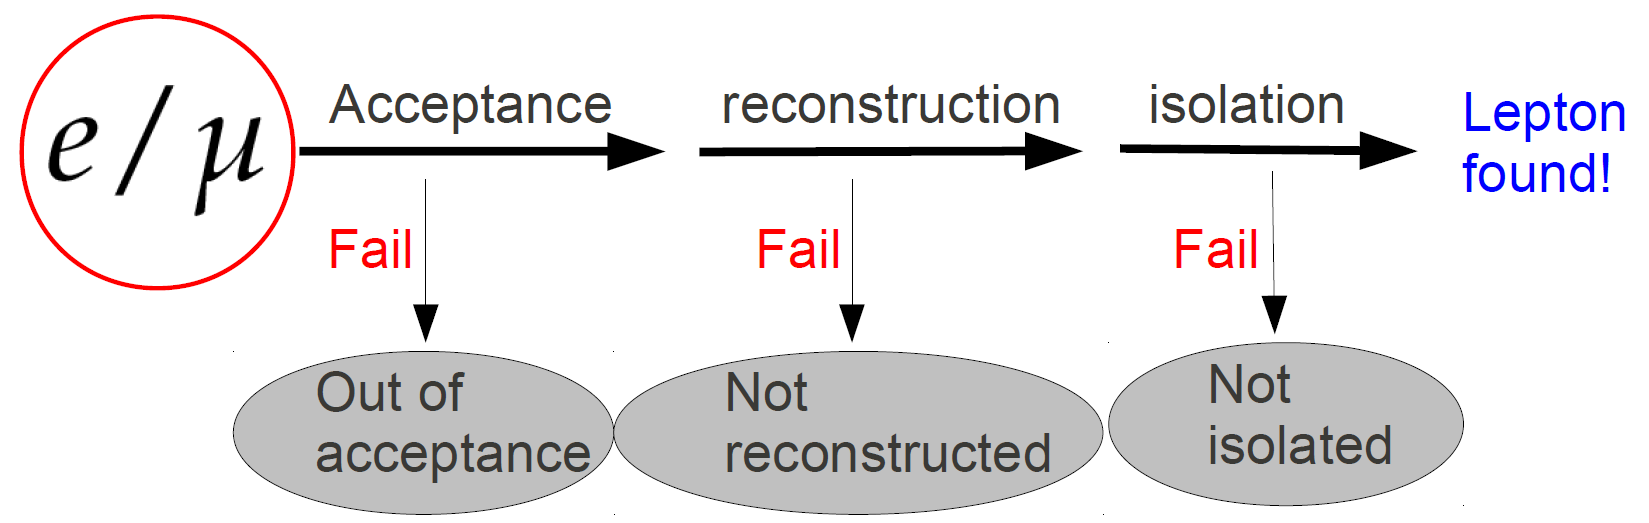
\includegraphics[width = 0.65\textwidth]{figures/lepton_veto_sketch.png}
%  \caption{Awesome figure}
 \end{figure}
      \begin{itemize}
      \item Select a control sample (CS) of exactly one well isolated $\mu$ within the acceptance
        \begin{itemize}
        \item Weight each CS event according to efficiencies for each identification step \\ (efficiencies determined from \ttbar and \wpj sample)
        \item Isolation and reconstruction efficiency in \HT, \MHT and \NJets parametrized
        \item Acceptance in \MHT and \NJets
        \end{itemize}
      \end{itemize}
\end{frame}
% --------------------------------------------------
\subsection{\mt cut }
\begin{frame}
\begin{itemize}
 \item Signal and other SM processes can contribute to $\mu$ control sample
 \item Suppress contamination by requiring trans. mass $\mt < 100 \gev$ \\
\end{itemize}

\frametitle{}
  \begin{columns}
    \begin{column}{0.6\textwidth}
    \begin{centering}
     $m_{T} = \sqrt{2 \cdot p_{T}(\mu)\cdot \met (1 - \cos(\Delta \Phi))}$
\end{centering}
      \begin{itemize}
      \item Removes about 15\% of $\mu$ CS
        \begin{itemize}
        \item Most of them di-leptonic \ttbar decays
        \item Mismeasured jets
        \item Highly virtual W
        \end{itemize}
      \begin{centering}
      \begin{overpic}[width=0.7\textwidth]{figures/MuMTWMHTNjet.pdf}
      \end{overpic}
      \end{centering}
      \item Correction as a function of \MHT \NJets applied
      \end{itemize}
    \end{column}
    \begin{column}{0.4\textwidth}
      \centering
      \begin{overpic}[width=0.8\textwidth]{figures/ControlSample__MTW__MCPrMTWDiLepTTbar+MCPrMTWDiLepW__mu_control_sample.pdf}
        \put(41.52,83){\color{black}\line(0,-1){67}}
    %    \put(6,39){\colorbox{white}{\textcolor{red}{\bf BSM decays?}}}
    %    \put(97,88){\rotatebox{-90}{\scriptsize CMS PAS HIG-14-009}}
    %    \put(13,2){\tiny assuming no tree-level modifications}
      \end{overpic}
      \begin{overpic}[width=0.8\textwidth]{figures/2012_ControlSample__MTW__Data_vs_TTbar+WJets__Baseline.pdf}
        \put(41.52,83){\color{black}\line(0,-1){67}}
    %    \put(6,39){\colorbox{white}{\textcolor{red}{\bf BSM decays?}}}
    %    \put(97,88){\rotatebox{-90}{\scriptsize CMS PAS HIG-14-009}}
    %    \put(13,2){\tiny assuming no tree-level modifications}
      \end{overpic}
    \end{column}
  \end{columns}
\end{frame}
% --------------------------------------------------
\subsection{di leptonic contribution}
\begin{frame}
\begin{itemize}
 \item The $\mt$ cut reduces di leptonic \ttbar contribution to the single $\mu$ control sample from ~5\% to about ~3\%
 \item But since the probability of losing two leptons is less likely than one di leptonic events are overestimated
 \item Separated estimation of lost di leptonic events applied
 \item Contribution to total amount of lost leptons ~1\%
\end{itemize}
  \begin{columns}
    \begin{column}{0.5\textwidth}
     \centering
      \begin{overpic}[width=0.95\textwidth]{figures/MuonDiLepMTW.pdf}
     \end{overpic}
    \end{column}
    \begin{column}{0.5\textwidth}
      \centering
      \begin{overpic}[width=0.95\textwidth]{figures/MuonDiLepEff.pdf}
      \end{overpic}
    \end{column}
  \end{columns}
\end{frame}
% --------------------------------------------------
\subsection{Closure}
\begin{frame}

Closure test for the lost lepton method:\\
\centering$\HT > 500 \gev, \MHT>200 \gev$, $\NJets\ge 3$ $\Delta\Phi_{1,2,3}>$0.5 0.5 0.3
  \begin{columns}
    \begin{column}{0.5\textwidth}
     \centering
      \begin{overpic}[width=0.6\textwidth]{figures/Closure__HT__MCPrMTWDiLep_vs_MCEx__csa_Baseline.pdf}
     \end{overpic}
           \begin{overpic}[width=0.6\textwidth]{figures/Closure__NJets__MCPrMTWDiLep_vs_MCEx__csa_Baseline.pdf}
     \end{overpic}
    \end{column}
    \begin{column}{0.5\textwidth}
      \centering
            \begin{overpic}[width=0.6\textwidth]{figures/Closure__MHT__MCPrMTWDiLep_vs_MCEx__csa_Baseline.pdf}
     \end{overpic}
      \begin{overpic}[width=0.6\textwidth]{figures/Closure__NVtx__MCPrMTWDiLep_vs_MCEx__csa_Baseline.pdf}
      \end{overpic}
    \end{column}
  \end{columns}
  \begin{itemize}
   \item Good closure can be observed for all search variables
   \item No pileup dependency visible
  \end{itemize}

\end{frame}
% --------------------------------------------------

\setcounter{framenumber}{14}

\end{document}
